\newpage
\section{Geschäftliche Grundlagen (10,75)}
\label{GeschäftlicheGrundlagen}
Das \ac{MMM} hat einen langen Weg zurückgelegt seit seiner Entstehung in den 1950er Jahren. \ac{MMM} hat sich mit der Verbreitung des digitalen Marketings weiterentwickelt. Später wurde \ac{MMM} durch die Fragmentierung der Media-Kanäle und den Signalverlust beeinflusst, die durch stetig wechselnde Datenschutz- und regulatorische Rahmenbedingungen verursacht werden \cite{MMMdef}.\\\\
In diesem Kapitel werden die geschäftlichen Grundlagen des \ac{MMM} im Bereich Media vorgestellt. Um den Nachfrageeffekt der Media-Kanäle zu berechnen, sind fachliche Grundlagen und Kenntnisse über die aktuelle Situation erforderlich. Zuerst werden Fachbegriffe wie Marketing-Mix-Modell, Medium, Werbeausgaben und Markenimage definiert. Bei Werbeausgaben wird auch auf die Entwicklung der Werbeausgaben hingewiesen, und der Zweck von Media-Kanälen im Kontext des Markenimages wird erläutert. Des Weiteren wird das Purchase-Funnel-Modell vorgestellt. Anschließend wird beschrieben, wie andere Unternehmen bei der Aufteilung der Mediaausgaben vorgehen. Zum Schluss wird die aktuelle Situation bei bonprix beschrieben und analysiert, um Verständnis bei der Modellierung zu verleihen und die Anforderungen dabei besser zu verstehen.
\subsection{Einführung in das Marketing-Mix-Modell}
\label{EinführungInDasMMM}
Das Marketing-Mix-Modell misst den Einfluss der Marketing-Aktivitäten auf die Nachfrage. Ein Marketing-Mix-Modell hilft einer Firma dabei, zukünftige Ausgaben und ihre Kapitalrendite (engl. \ac{ROI}, Return on Investment) zu maximieren. Dabei misst das \ac{MMM} alle möglichen Marketingeffekte und deckt die Marketinginvestitionen auf, die ein langfristiges Ertragswachstum erzielen. Das sind die Variablen, die Marketing-Manager kontrollieren, um den Verkauf in der Firma zu beeinflussen. \\\\Das Fachwort \textit{Mix} in \ac{MMM} referiert die klassischen \textit{4Ps} im Marketing: Product, Price, Place and Promotion (Engl. Produkt, Preis, Ort und Verkaufsförderung)\cite[S. 109 ff]{akinkunmi2018data}. \\\\
Produkt steht für die Produkte der Firma und warum sie aus den Konkurrenzprodukten ausstechen. Darunter werden beispielsweise hohe Qualität, äußerliche Erscheinung und Wartung verstanden. Werbung bedeutet die Darstellung der Produkte seitens der Firma mithilfe von Werbungen, Gutscheinen, Handelsmessen etc. Der Preis umfasst die Preisstrategien, die in Verbindung zur Produktpalette der Firma stehen. Diese hängen von dem Produkt-Lebenszyklus, den Produkteigenschaften, dem wahrgenommenen Nutzen und der Konkurrenz ab. Ort beschreibt den Zustellungsbereich der Produkte quantifiziert durch die Variablen wie Distribution, Verfügbarkeit und Bequemlichkeit\cite{akinkunmi2018data}. Das \ac{MMM} wird in \autoref{fig:mmm} visualisiert. \\\\ 
\begin{tikzpicture}[node distance=5.2cm, auto, centered]

\node (target) [ellipse, draw, text centered, minimum width=4cm, minimum height=2cm, text width=3.5cm] {ZIELMARKT};
\node (product) [ellipse, draw, above left of=target, text centered, minimum width=3cm, minimum height=2cm, text width=4cm] {Produkt \\ Was soll produziert und verkauft werden};
\node (place) [ellipse, draw, above right of=target, text centered, minimum width=3cm, minimum height=2cm, text width=3.5cm] {Ort \\ Wo soll das Produkt verkauft werden};
\node (promotion) [ellipse, draw, below left of=target, text centered, minimum width=3cm, minimum height=2cm, text width=6cm] {Werbung \\ Werbung, persönliche Verkaufsförderung, Verkaufsaktionen und Öffentlichkeitsarbeit};
\node (price) [ellipse, draw, below right of=target, text centered, minimum width=3cm, minimum height=2cm, text width=3.5cm] {Preis \\ Wie viel soll das Produkt kosten};

\draw[->] (product) -- (target);
\draw[->] (place) -- (target);
\draw[->] (promotion) -- (target);
\draw[->] (price) -- (target);


\node[below=1cm of promotion, text centered] {Abbildung 1: Marketing-Mix-Modell (\ac{MMM}) mit den vier P's \cite{akinkunmi2018data}};
\label{fig:mmm}

\end{tikzpicture}
Die Entwicklung des \ac{MMM}s wurde geprägt durch die Suche nach der optimalen Allokation der Marketingausgaben. Darunter werden Fragen gestellt wie: Was für eine Kombination von Marketing-Mix-Variablen maximiert die Ausgaben wie Unternehmensumsatz oder Marktanteil am Gewinn? Wie reagieren diese auf die Ausgaben dieser Marketing-Mix-Variablen? Darauffolgend haben Forscher ein wirtschaftliches Modell entwickelt, das diese Problematik behandelt. Das \ac{MMM} verwendet vergangene Daten, um valide Konklusionen zu erstellen und bessere Marketingstrategien für die Zukunft zu entwickeln.\\\\
In der heutigen Zeit wird das Bestimmen des effizientesten Marketing-Mix komplexer aufgrund der neuen Marketingstrategien und der Komplexität von computergestützten Daten. Das \ac{MMM} verwendet häufig multiple Regressionsmodelle, um die optimale Kombination der Marketing-Mix-Variablen vorherzusagen. Der Einsatz eines Regressionsmodells unterstützt dabei, den Einfluss unabhängiger Variablen wie Verkaufsförderung und Werbekosten auf die abhängige Variable, beispielsweise die Nachfrage, zu analysieren \cite{akinkunmi2018data}.\\\\
Ein entwickeltes Regressionsmodell beschreibt die Beziehung zwischen den Variablen und kann eingesetzt werden, um den zukünftigen Verkauf vorherzusagen. Das Modell kann auch identifizieren, welche Koeffizienten der unabhängigen Variablen einen starken Einfluss auf den Kaufwunsch der Kunden haben. Unterschiedliche Eingabe-Variablen für das \ac{MMM} können verwendet werden. Dazu gehören wirtschaftliche Daten wie Zinsrate, Inflationsrate, industrielle Daten wie der Preis, Konkurrenz und Services, Marktdaten wie Verkauf, Umsatz, Gewinn und \ac{ROI} und zum Schluss noch die Zielgruppendaten. Normalerweise hängt die Stabilität des Modells mit der Genauigkeit der Daten zusammen. 

\subsection{Medium Definition}
\label{Media-KanäleDefinition}
Media wird definiert durch Kommunikationsträger. Insbesondere Massenmedien ermöglichen es dem Kommunikator, einen größeren Empfängerkreis zu erreichen. Der Empfängerkreis ist zeitlich und räumlich von sich und von dem Kommunikator getrennt, aber durch die gemeinsame Zuwendung zum Medium wird er erreicht. Klassische Massenmedien bedürfen typischerweise physischer Medien wie Zeitungen, Hörfunk und Zeitschriften. Durch die Digitalisierung entstehen digitale Kommunikationsträger wie soziale Medien und Blogs. Diese ermöglichen einen \anf{viele zu vielen}-Austausch, dass Individuen und Unternehmen im Netzwerk gleichberechtigt kommunizieren. Diese Medienmodelle sind für das Unternehmen von Interesse, da sie innerhalb kurzer Zeit einseitig an ein großes Empfängerpublikum adressiert werden können. Sie treten beispielsweise in Form von Werbe- und \ac{PR}-Kampagnen auf \cite{Kleinjohann2024}. \ac{PR} steht für nahezu Öffentlichkeitsarbeit auf Englisch und bezeichnet die Kommunikation zwischen Organisationen oder Personen mit deren Umwelt. Dabei wird der Beziehungsaspekt zwischen den Beteiligten hervorgehoben \cite{Büsching2014}. \\\\
\subsection{Werbeausgaben}
\label{werbeausgaben}
Werbeausgaben sind Ausgaben eines Unternehmens, um auf einer Werbefläche ihre Produkte oder Dienstleistungen zu bewerben. Diese werden in zwei Hauptkanäle, traditionelle Werbung und digitale Werbung, umfasst. Die traditionelle Werbung wird definiert durch die Above-the-Line-Medien, die die Werbebotschaften einem breiten Publikum übermitteln. Die Above-the-Line-Medien umfassen Massenmedien wie traditionelles Fernsehen, traditionelles Radio, gedruckte Zeitungen, Magazine und Out-of-Home-Werbeformate. Zur digitalen Werbung gehören Medien, die über das Internet ihre Werbebotschaften an Internet-Nutzer übermitteln. Darunter fallen digitale Out-of-Home-Werbungen, digitale Werbebanner, digitale Audiowerbung, digitale Kleinanzeigenwerbungen, Werbungen in digitalen Videos und Suchmaschinen sowie Influencer-Werbung. Die Werbeausgaben für Deutschland in 2025 werden auf 25,93 Milliarden Euro geschätzt, was einer Steigerung von 2,93 \% im Vergleich zum Vorjahr entspricht \cite{statista_werbung}. Werbeausgaben der Media-Kanäle beziehen sich auf Werbeausgaben für Werbefläche in einem Medium. Da bonprix bestimmte Media-Kanäle intern definiert hat, werden nur diese in dieser Arbeit ausführlich beschrieben. \\\\ 
Wie in der \autoref{fig:statistawerbungde} dargestellt, werden die Werbeausgaben in Deutschland aufgeteilt. Dieses von Statista Insights geführte Balkendiagramm visualisiert die Verteilung der Werbeausgaben und deren Entwicklung in Deutschland. Im Jahr 2025 wird die Suchmaschinenwerbung mit 6,92 Milliarden Euro an erster Stelle stehen. Darauf folgt die TV- und Videowerbung mit 5,64 Milliarden Euro, gefolgt von der digitalen Bannerwerbung mit 3,26 Milliarden Euro. Die TV- und Videowerbung wird noch aufgeteilt in 1,53 Milliarden Euro in digitale Videowerbung und 4,12 Milliarden Euro in traditionelle TV-Werbung. Als Trend wird in Deutschland im Jahr 2029 63 \% der Werbeausgaben im digitalen Bereich erwartet und voraussichtlich 83 \% der Werbeausgaben entfallen auf Programmatic. Der Werbemarkt in Deutschland hat in den letzten Jahren ein starkes Wachstum verzeichnet. Laut einer Analyse von Statista (2024) haben verschiedene Faktoren wie Kundenpräferenzen, Markttrends, lokale Besonderheiten und makroökonomische Gegebenheiten maßgeblich zur Entwicklung dieses Marktes beigetragen. Insbesondere legen deutsche Verbraucher großen Wert auf Qualität und Authentizität, wobei personalisierte Werbung zunehmend an Bedeutung gewinnt. Gleichzeitig beeinflussen die zunehmende Digitalisierung und der Trend zu Influencer-Marketing das Werbeverhalten. Statista (2024) hebt hervor, dass auch der starke Fokus auf Datenschutz und die wachsende Bedeutung von Online-Werbung den Markt prägen \cite{statista_werbung}.
\begin{figure}[H]
    \centering
    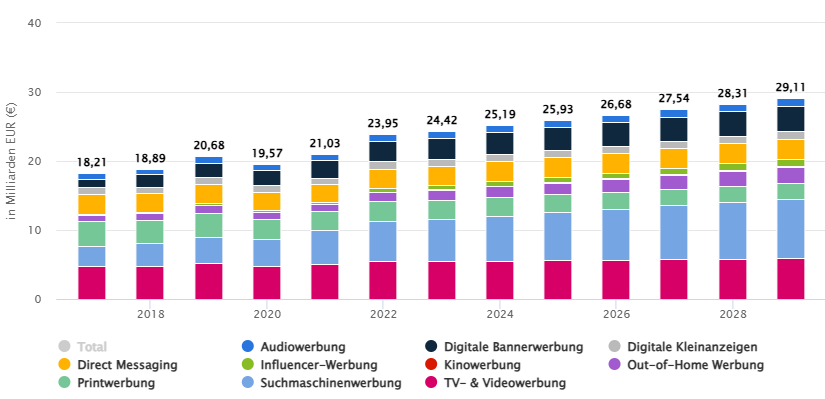
\includegraphics[width=0.90\linewidth]{images/werbede.png}
    \caption{Dokumentierte und geschätzte Werbeausgaben in Deutschland \cite{statista_werbung}}
    \label{fig:statistawerbungde}
\end{figure}
\subsection{Markenimage}
\label{markenimage}
Nach dem Prozess der subjektiven Wahrnehmung und Dekorierung aller Kommunikationsbotschaften zur Marke entsteht das Markenimage als Fremdbild einer Marke. Der Botschaftsempfänger bewertet dabei die Eignung der Marke und die Befriedigung seiner Bedürfnisse. Anders als die Markenidentität wird das Markenimage nicht vom Management gesteuert. Das Markenimage wird beeinflusst von Aktivitäten der Markenführung und anderen Einflüssen \cite{burmann2024}. \\\\
Das Markenimage wird definiert durch \anf{ein mehrdimensionales Einstellungskonstrukt, welches das in der Psyche externer Nachfrager fest verankerte, verdichtete und wertende Vorstellungsbild einer Marke
wiedergibt}  \cite{burmann2024}.\\\\
Voraussetzung für ein Markenimage ist die Bekanntheit einer Marke. Markenbekanntheit misst die Fähigkeit, sich an eine Marke zu erinnern. Ungestützte Markenbekanntheit (Brand Recall) ist das Erinnern an ein Markenzeichen wie Wortmarke, Bildmarke oder Wort-Bild-Marke. Gestützte Markenbekanntheit (Brand Recognition) ist das Erkennen der Marke nach einer akustischen und/oder visuellen Stützung. Da Markenbekanntheit eine Voraussetzung des Markenimages ist, ist sie kein Bestandteil eines Markenimages \cite{burmann2024}. \\\\
Aus ökonomischer Sicht verringern Marken die Such- und Informationskosten. Eine Marke kann für die Kunden deshalb \anf{günstiger} sein. Aus Sicht des Kundenverhaltens dient die Marke zur Orientierung. Die Marke erhöht die Markttransparenz, dadurch identifizieren Kunden schneller und einfacher die für sie passenden Angebote \cite{burmann2024}.  
\subsection{Purchase-Funnel-Modell}
\label{PurchaseFunnelModell}
Das Purchase-Funnel-Modell beschreibt den trichterförmigen Verkaufsprozess. Das Purchase-Funnel-Modell ist eine Anlehnung an das AIDA-Modell. Das AIDA-Modell geht auf Lewis im Jahr 1899 zurück und beschreibt den Ablauf der Werbekommunikation in vier Stufen. Die Stufen sind jeweils Aufmerksamkeit (Attention), Interesse (Interest), Verlangen (Desire) und Kauf (Action). Wie das AIDA-Modell bildet das \anf{Purchase Funnel}-Modell ebenfalls ein Stufenmodell von der Kontaktaufnahme bis zum Kaufabschluss. Das \anf{Purchase Funnel}-Modell wird generell in \anf{oberen Trichter}, \anf{mittleren Trichter} und \anf{unteren Trichter} aufgeteilt. Sie werden jeweils abgekürzt als \ac{ToFu}, \ac{MoFu} und \ac{BoFu}. Sie sind vergleichbar mit den Phasenzielen des AIDA-Werbewirkungsmodells mit Aufmerksamkeitsgenerierung (Awareness), Interessensweckung (Interest) und Kauf (Action) \cite{Kleinjohann2024}. \\\\
Im oberen Teil des Trichters \ac{ToFu} wird der Konsument auf sein Problem oder Bedürfnis aufmerksam. Er sucht Lösungen in Form von Produkten und richtet sein Interesse auf das verfügbare Marktangebot. Im mittleren Teil des Trichters \ac{MoFu} bewertet der potenzielle Käufer das Angebot und nimmt Kontakt mit dem Anbieter auf oder nähert sich dem Verkaufsort. Im unteren Teil des Trichters \ac{BoFu} trifft der Konsument die Entscheidung, welches Produkt seine Bedürfnisse befriedigt und kauft es \cite{Kleinjohann2024}.\\\\
Im digitalen Verkaufsprozess wird der Verkaufstrichter ein \anf{Conversion Funnel} und wird erweitert. Im \ac{ToFu} verknüpft die digitale Kommunikation wie \ac{SEA}, Content Marketing und E-Mail qualifizierte Kontakte zwischen Unternehmen und potenziellen Verkäufern \cite{Kleinjohann2024}. \ac{SEA} ist die Praxis von einem Unternehmen, für die Suchmaschinenwerbung zu bezahlen und Keywords zu buchen \cite{Bartholomew2005MakingAM}. 
\begin{figure}[H]
    \centering
    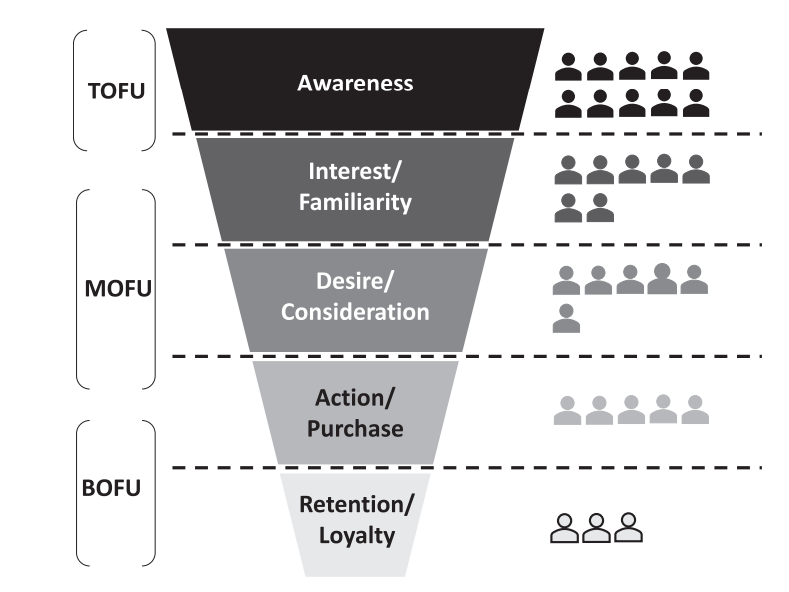
\includegraphics[width=0.75\linewidth]{images/Funnel.png}
    \caption{Purchase-Funnel-Modell \cite{Kleinjohann2024}}
    \label{fig:purchase-funnel}
\end{figure}
\subsection{Media-Kanäle in der Praxis}
\label{MediaKanäleInDerPraxis}
Mit wachsenden Kosten in Media-Kanälen gewinnt die Aufteilung der Kosten pro Kanal an Bedeutung. \\\\
Die Versicherung Generali hat in 2022 in ihrem \ac{MMM} herausgefunden, dass YouTube im Vergleich zu anderen Media-Kanälen überproportional stark auf die Steigerung von Markenbekanntheit, Markenpräferenz und Versicherungsabschlüssen einwirkt\cite{DasZusammenspielKundenloyalität2022}. Die Nutzer sollen während des Lockdowns gelernt zu haben, YouTube als Erklärinhalte zu nutzen. So hat die YouTube-Werbung alle gemessenen Loyalitätsmetriken von der Versicherung positiv beeinflusst. 44 \% der Nutzer, die solche Videos gesehen haben, kategorisieren die Versicherung als ihre erste Wahl. 15 \% mehr Nutzer zogen einen Anbieterwechsel in Betracht und 6 \% mehr Nutzer sprachen für eine Weiterempfehlung aus\cite{DasZusammenspielKundenloyalität2022}. \\\\
Ein weiterer Bericht thematisiert den Wandel der Media-Kanäle. Eine von Nielsen im Auftrag von Google durchgeführte Metaanalyse zeigt, dass YouTube ein Effektivitätstreiber ist und das lineare TV beim \ac{ROI} (Engl. Rentabilität der Investition) übertrifft. Das Nutzungsverhalten für Media wird fragmentierter und das TV verliert an Bedeutung. Bei Personen unter 40 beträgt die Nutzung von linearem TV inzwischen weniger als 50 \% der gesamten Bewegtbildnutzung \cite{237097}.\\\\
Die Ergebnisse zur Abverkaufswirkung aus 144 \ac{MMM} wurden untersucht. Dabei zeigt sich, dass vier von fünf Unternehmen von höheren YouTube-Ausgaben in ihrem Marketing-Mix profitieren würden, um den Bewegtbild-ROI für TV und YouTube zu maximieren\cite{237097}. \\\\
Auch Offline-Medien haben eine Auswirkung auf das Kaufverhalten. Die zentrale Marktforschungsfirma von Deutschlands größter Mediaagenturgruppe, M-Science, brachte im Mai 2019 das Tool \anf{Crossoptimiser} zur Welt. Das Tool behandelt das Problem der Wirkungsforschung, dass manche Einflussfaktoren auf das Werbeergebnis übersehen werden. Die gängigen Modelle ordnen messbare Erfolge allein Online-Kanälen zu. Beispielsweise werden die Bekanntheit, generierte Adressen und Kaufabschlüsse dem letzten Werbeklick der Nutzeraktivität im Netz honoriert. Dieser Schluss übersieht die Wirkungsbeiträge, die Offline-Medien zu einem früheren Zeitpunkt im Wahrnehmungs- und Verkaufsprozess leisten. Vergleichbar mit dem Marketingtrichter, Nutzer finden und bestellen online Produkte, weil sie früher eine Print- oder TV-Werbung gesehen haben. Karin Immenroth, die Geschäftsführerin und zugleich Marktforscherin der Group M, zieht ihre ersten Schlussfolgerungen nach einem Jahr Vorarbeit und hunderten durchgerechneten Kampagnen. Ihre Schlussfolgerungen besagen, gerade bei Kunden mit einem hohen digitalen Werbeanteil wird der Wirkungsbeitrag von Offline oft stark unterschätzt. Je weiter sie im Marketingtrichter zurückforschen, desto stärker zeigt sich der Einfluss von Offline-Medien. Besonders bei Marken mit noch relativ niedrigen Awareness-Werten \cite[S. 4]{20190411492848}.
\\\\
Jollibee Food Corporation wurde 2020 die größte Fast-Food-Kette auf den Philippinen. Während einer Gesundheitskrise fiel der Verkauf im ersten Quartal um 10~\%. Um den Verkauf zu unterstützen, strebte das Unternehmen einen optimalen Media-Mix an. Es berichtete die gewertete Exposition der fünf üblichen Medien: TV, Magazin, lokale Zeitung, Plakat (\ac{ooh}) und soziale Medien. Jollibee gibt jährlich 9 bis 12~\% des Budgets für Werbung aus. Dabei werden die Kosten für lokale Zeitungen und Magazine kombiniert und auf unter 20~\% begrenzt. Zudem darf kein einzelner Kanal mehr als 30~\% des Budgets beanspruchen. Die Zielgruppen wurden in Haushalte mit niedrigem, mittlerem und hohem Einkommen unterteilt, mit Mindestwerten für erreichte Personen pro Peso je Medium. Mithilfe von Constraints wie maximalen Kosten wurde die optimale Kombination für eine maximale Gesamt-Reichweite mit einem Excel-Solver berechnet \cite{Tapiceria2020}. \\\\
Eine optimale Verteilung der Media-Kanäle kann dabei das maximale Potenzial jedes Kanals ausschöpfen. Denn Unternehmen, die in wirtschaftlich herausfordernden Zeiten mit geprüfter und gesteigerter Effizienz der Maßnahmen in das Marketing investieren, sind überdurchschnittlich erfolgreich \cite{237097}. \\\\ 
\subsection{Marketing-Mix-Modell bei bonprix} 
\label{Marketing-Mix-ModellBeiBonprix}
Bei bonprix modelliert das Marketing-Mix-Modell Daten ab 2020. \\\\
Vor der Entstehung des \ac{MMM} haben unterschiedliche Bereiche und Verantwortliche eigene Bewertungsansätze formuliert, um den jeweiligen Nachfrageeffekt zu bewerten. Beispiele für diese Bereiche sind Online-Marketing, Katalog und Media. Dabei wurde der Nachfrageeffekt der anderen Bereiche nicht berücksichtigt, und verschiedene Ansätze erschweren den direkten Vergleich der Kennzahlen. Zudem wurden die einzelnen Ländervertriebe organisatorisch zusammengeführt, um eine optimale Marketing-Budget-Strategie für ganz Europa zu erarbeiten. Es gab ein Bestreben, die Bewertungsansätze für den Nachfrageeffekt der Marketing-Bereiche zu vereinheitlichen. Hierbei soll das Marketing-Mix-Modell helfen. Das Marketing-Mix-Modell soll die Budgetentscheidungen unterstützen und zu einer besseren Verteilung des Budgets über die Länder hinweg beitragen.\\\\
\begin{figure}[H]
    \centering
    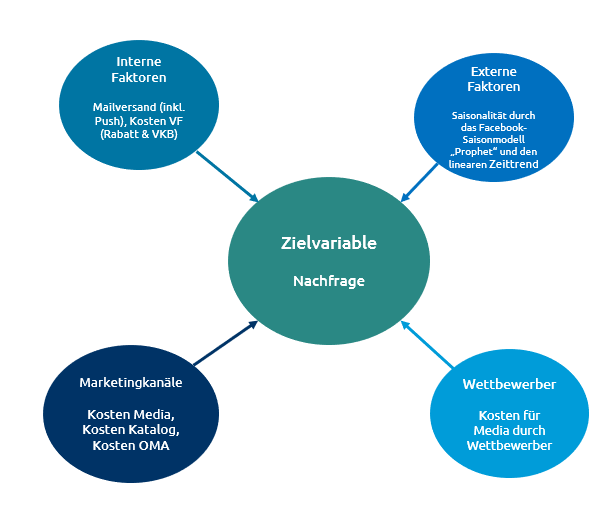
\includegraphics[width=0.85\linewidth]{mmm.png}
    \caption{Marketing-Mix-Modell bei bonprix, eigene Darstellung}
    \label{fig:mmmbonprix}
\end{figure}
Das Marketing-Mix-Modell von bonprix berechnet den \ac{ROAS} für jeden Marketing-Kanal. \ac{ROAS} steht für die Nachfragesteigerung, die der Werbung zugeordnet werden kann \cite{roas}:
\begin{equation}
ROAS = \frac{\text{Nachfragesteigerung, die der Werbung zugeordnet werden kann} \, (Euro)}{\text{Werbeausgaben} \, (Euro)}
\end{equation}
Jedes Jahr geben Marketer Milliarden von Dollar für Online-Werbungen aus, um das Verhalten der Kunden zu beeinflussen. Die Online-Werbungen haben einen Vorteil. Sie quantifizieren Kundenverhalten, das mit den Online-Werbungen verbunden ist. Das heißt, bezahlte Klicks, Website-Besuche und verschiedene Arten von Conversions können gesammelt werden. Allerdings sagen diese Kennzahlen nicht aus, wie sich die Kunden verhalten, wenn es die Werbung nicht gegeben hätte. Um die Werbung zu verstehen, ist es wichtig, die Verhaltensänderung zu messen \cite{roas}. Zu diesem Anlass wird der ROAS als Kennzahl für den Werbeeffekt eingesetzt. \\\\
Wie in \autoref{fig:mmmbonprix} beschrieben, werden unabhängige Variablen genutzt, um die Zielvariable \anf{Nachfrage} zu beeinflussen. Das Modell ähnelt dem in \autoref{EinführungInDasMMM} beschriebenen Modell. Die Variablen werden in vier Bereiche unterteilt: interne Faktoren, externe Faktoren, Marketingkanäle und Wettbewerber. Für die internen Faktoren verwendet das Modell Variablen wie Aktionen und Mailversand. Das bedeutet, dass Verkaufsförderungen wie Rabatte, Versandkostenbefreiungen und die Anzahl an E-Mails, wie Newsletter und Trigger, genutzt werden. Für die externen Faktoren stehen die Saisonalität und der lineare Zeittrend zur Verfügung. Bonprix verwendet eine Schätzung von Meta, die die Saisonalität des Konsums vorhersagt. Für den linearen Zeittrend wird das Datum in fortlaufende Tage umgewandelt, wie Tag 1, Tag 2, ..., Tag n. Denn das \ac{MMM} kann kein Datum interpretieren, sondern verwendet den Zeitverlauf als fortlaufende Zahlen. Für die eigenen Marketingkanäle werden Ausgaben von anderen Kanälen berücksichtigt. Bonprix investiert in das Online-Marketing \ac{OMA}, in Medienkanäle und in Kataloge. Da bonprix früher mit Katalogen geworben hat und es immer noch Leser gibt, investiert bonprix weiterhin in Kataloge. Das Online-Marketing ist ein führender Kanal. Täglich entstehen Kosten für das Online-Marketing, und es hat auch vergleichsweise einen großen Einfluss auf die Nachfrage. In 
\autoref{tab:mmmausgaben} ist zu erkennen, dass nach dem \ac{MMM} das Online-Marketing als steuerbarer Einflussfaktor den größten Einfluss auf die Nachfrage hat. Im ersten Zeitfenster, vom 1. Quartal 2020 bis zum 4. Quartal 2021, werden 36,5 \% der Nachfrage durch das Online-Marketing erklärt. Im Zeitraum vom 3. Quartal 2020 bis zum 2. Quartal 2022 sind es 29,8 \%, und im Zeitraum vom 1. Quartal 2021 bis zum 4. Quartal 2022 sind es 18 \%. Diese Werte werden abgeschwächt, da bonprix eine Sättigungsfunktion verwendet. Ab einer bestimmten Höhe der Ausgaben steigt die Nachfrageänderung langsamer, wodurch die ROAS für das Online-Marketing realistisch angepasst werden. Ferner besteht Media aus verschiedenen Unterkanälen, die in dem \nameref{MediaKanäleBeiBonprix} ausführlicher beschrieben werden. Abschließend werden die Werbeausgaben von vier Konkurrenten im Bereich Online-Mode berücksichtigt.\\\\
Außer der Sättigungsfunktion werden auch andere Mechanismen verwendet, um die \ac{MMM}-Daten an Realität angepasst zu transformieren. Denn Werbeausgaben wirken nicht sofort und ihre Wirkung nimmt über die Zeit hinab. Der Carry-Over-Effekt (Adstock) wird integriert. Sie quantifiziert den verlängerten oder verzögerten Effekt von Werbung auf das Kaufverhalten der Verbraucher \cite{broadbent1979}. Adstock ist ein wichtiges Komponent des \ac{MMM}. Auch der Abklingeffekt wird modelliert. Denn nach der Exposition einer Werbung wird das Bewusstsein für die Marke erhöht, jede neue Werbeeinblendung steigert das Bewusstsein auf ein neues Niveau. Der Abklingeffekt reduziert das Bewusstsein bis zum Basisniveau, es sei denn der Abklang wird verlangsamt oder gestoppt von erneuten Werbeeinblendungen \cite{Joseph2006Adstock}. Nach der Transformation wird ein Modell trainiert. Für das \ac{MMM} wird die robuste Huber-Regression verwendet, um den \ac{ROAS} zu berechnen. Die Huber-Regression wird im \autoref{huberregression} detaillierter erklärt. Während der Entwicklung von \ac{MMM} wurden auch andere Modelle ausprobiert. Allerdings waren die Ergebnisse nicht zufriedenstellend, und aufgrund des nachvollziehbaren Konzepts sowie der besseren Ergebnisse wird die Huber-Regression für die Berechnung des \ac{ROAS} beibehalten.
\begin{table}[H]
\centering
\renewcommand{\arraystretch}{1.3}
\setlength{\tabcolsep}{10pt}
\begin{tabular}{|l|c|c|c|}
\hline
\textbf{Einflussfaktor} & \textbf{Q1-20/Q4-21} & \textbf{Q3-20/Q2-22} & \textbf{Q1-21/Q4-22} \\ \hline
OMA                    & 36,5 \%               & 29,8 \%               & 18,0 \%               \\ \hline
Katalog                & 8,7 \%                & 8,4 \%                & 7,2 \%                \\ \hline
Media                  & 0,5 \%                & 1,5 \%                & 1,6 \%                \\ \hline
Mail                   & 2,5 \%                & 4,2 \%                & 3,0 \%                \\ \hline
Rabatt                 & 10,1 \%               & 13,1 \%               & 15,4 \%               \\ \hline
VKB                    & 6,6 \%                & 4,7 \%                & 4,7 \%                \\ \hline
Externe Faktoren       & 14,2 \%               & 19,7 \%               & 27,6 \%               \\ \hline
Konstante              & 21,0 \%               & 18,6 \%               & 22,5 \%               \\ \hline
\end{tabular}
\caption{\ac{MMM}-Ausgaben-Tabelle mit überlappenden Zeitfenstern von jeweils ungefähr zwei Jahren, eigene Darstellung}
\label{tab:mmmausgaben}
\end{table}
\subsection{Media-Kanäle bei bonprix} 
\label{MediaKanäleBeiBonprix}
Die Media-Ausgaben waren zu Beginn der \ac{MMM}-Entwicklung sehr gering, weshalb die Effizienzanalyse ihrer Unterkanäle vernachlässigt wurde. \\\\
Im \ac{MMM} von bonprix nehmen die Media-Ausgaben nur einen kleinen Anteil der Gesamtkosten ein. Der Kostenanteil von Media wird im Folgenden mit etwa zweijährigen, überlappenden Zeitfenstern betrachtet: Zwischen dem ersten Quartal 2020 und dem vierten Quartal 2021 betrugen die Media-Ausgaben 0,5 \%. Sie stiegen im nächsten Zeitraum, vom dritten Quartal 2020 bis zum zweiten Quartal 2022, auf 1,5 \%. Zum Schluss erhöhten sich die Media-Ausgaben vom ersten Quartal 2021 bis zum vierten Quartal 2022 auf 1,6 \%. Um die Media-Ausgaben mit den Kosten anderer Kanäle zu vergleichen, werden alle Kosten als Anteil in Form von einem Balkendiagramm in \autoref{fig:mmmdiagramm} visualisiert. 
\begin{figure}[H]
    \centering
    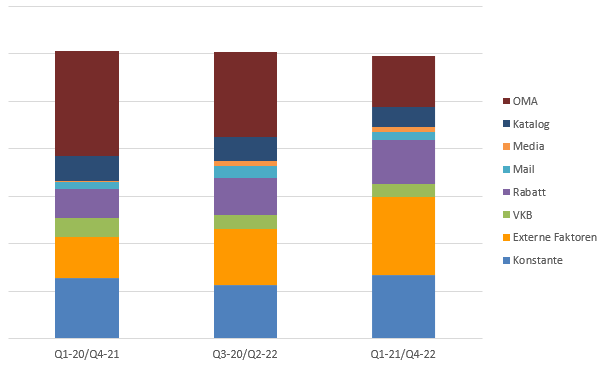
\includegraphics[width=0.75\linewidth]{images/mmmdiagramm.png}
    \caption{Nachfrageeffekt je Einflussfaktor aus dem \ac{MMM}-Modell, eigene Darstellung }
    \label{fig:mmmdiagramm}
\end{figure}
\noindent
Bei bonprix werden Mediaausgaben in Kampagnen umgesetzt. Das bedeutet, dass Media-Schaltungen aktiviert werden, wenn Kaufsaison ist und die Nachfrage hoch ist. Media-Schaltungen werden eingesetzt, um die maximale Reichweite beim Publikum zu erzielen. Die Dauer für die Aktivierung eines Media-Kanals ist ebenfalls begrenzt. Für das Online-Marketing fallen täglich Kosten an. Im Gegensatz zum Online-Marketing wird ein Media-Kanal nur für einen begrenzten Zeitraum, wie einen Monat oder zwei Wochen, aktiviert. Normale Kampagnen dauern vier Wochen. Radio wird zwei Tage bis maximal zwei Wochen aktiviert. \\\\
Der Media-Mix wird anhand der Zielstellung der Kampagnen (Awareness oder Consideration, s. \nameref{PurchaseFunnelModell}) abgeleitet. Ein Medium hat einen bestimmten Werbedruck und ein begrenztes Budget. Werbedruck wird definiert durch die Sichtbarkeit eines Unternehmens im Vergleich zu seinen Konkurrenten. Pro Jahr werden vier Kampagnen durchgeführt. In jeder Jahreszeit, Frühling, Sommer, Herbst und Winter, findet jeweils eine Kampagne statt. Diese Kampagnen erfolgen jeweils zwischen März und April, Mai und Juni, September und Oktober sowie Oktober und November. Radio wird zum Beispiel zu bestimmten Aktionen wie Valentinstag, Rabattaktionen aktiviert.\\\\
Die Anforderung für die Aufteilung der Mediaausgaben ist die Reichweite bei der Zielgruppe. Die Zielgruppe von bonprix sind 30-59-Jährige. Mindestens 70\% der Zielgruppe sollen pro Medium erreicht werden. Normalerweise wird diese Grenze überschritten. Außerdem wird der Werbedruck analysiert. Es wird beobachtet, wie viele Media-Schaltungen die Konkurrenten schalten, um weitere eigene Media-Schaltungen zu aktivieren. Dabei wird auf die eigene Sichtbarkeit eingegangen. Im \nameref{PurchaseFunnelModell} zielen Medienkampagnen darauf ab, zum \ac{ToFu} und \ac{MoFu} beizutragen. Das bedeutet, dass potenzielle Kunden auf die Marke aufmerksam werden und die Medienkampagnen ihr Interesse wecken sollen. \\\\
In der Media-Abteilung werden bereits \ac{KPI}s verwendet. Dazu zählen gestützte und ungestützte Markenbekanntheit (Brand Awareness), Markenberücksichtigung (Consideration) und Werbeerinnerung (Ad Recall). Die fachlichen Grundlagen werden in \nameref{markenimage} und \nameref{PurchaseFunnelModell} beschrieben. Im \ac{MMM} wird auch der \ac{ROAS} gerechnet. Allerdings wird das Medium als Ganzes betrachtet und nicht auf die einzelnen Kanäle wie TV, \ac{dooh}/\ac{ooh}, Radio usw. heruntergebrochen. Der ROAS wird im Unternehmen für die übergeordnete Budgetplanung berücksichtigt, jedoch fehlen spezifische Daten, um ihn für die konkrete Mediaplanung einzusetzen. Um den ROAS für die einzelnen Media-Kanäle zu berechnen, wird ein neues Modell entwickelt. Daher wird ein neues Modell entwickelt, das die Reichweite der Media-Schaltungen vorhersagen soll. Diese Entwicklung findet außerhalb, aber parallel zu dieser Arbeit statt. Dennoch ist es wichtig zu untersuchen, ob Media-Kanäle die Nachfrage positiv beeinflussen und somit Entscheidungen unterstützen können. Daraus ergibt sich die Forschungsfrage, und der Kern dieser Arbeit ist das Erforschen des Nachfrageeffekts der Media-Kanäle. Das Ergebnis dieser Arbeit soll eine Erweiterung des \ac{MMM} dienen. Die Huber-Regression soll verwendet werden, um den \ac{ROAS} der Media-Kanäle im \ac{MMM} weiter zu berechnen. \\\\
In den Daten von \ac{MMM} sind auch die Kosten der jeweiligen Media-Kanäle enthalten. Jedoch werden Media-Schaltungen nicht nur aktiviert, wenn Kosten in den Daten anfallen. Ein Anbieter wie ProSieben bietet beispielsweise auch kostenlose Werbespots an, wenn bestimmte Ausgaben erreicht werden. Das heißt, ungefähr 90\% der Media-Schaltungen werden mit Kosten dokumentiert und 10\% der Media-Schaltungen werden in den \ac{MMM}-Daten nicht mehr berücksichtigt. Die Nachfrageeffekte von diesen 10\% der Media-Schaltungen werden in dieser Arbeit nicht mehr analysiert. \\\\
Es existieren Herausforderungen bei dem Messen des Werbeeffekts für Media. Für TV wird ein Tool eingesetzt, das die Webshop-Besuche nach einer TV-Werbung zählt. Dabei wird die Erhöhung des Traffics im Webshop erkannt. Für die Online-Werbungen ist es auch möglich, die Veränderung der Besucheranzahl zu dokumentieren. Jedoch ist es schwieriger, die Reichweite für \ac{dooh}, \ac{ooh} und Radio zu messen. Als \ac{KPI} für \ac{dooh}, \ac{ooh} und Radio wird die prognostizierte Reichweite herangezogen.